% Analysis paper draft -- compile in Overleaf (acmart is preinstalled there).
% Upload the whole paper/ folder: main.tex, references.bib, figures/, tables/.
% Every number below comes from method_paper/EXPERIMENT_LOG.md; figures and
% Table 1 are regenerated by `python paper/make_figures.py`.
%
% Status markers: \todo{...} = still to write or verify.
\documentclass[sigconf,review,anonymous]{acmart}

\usepackage{booktabs}
\usepackage{xcolor}
\newcommand{\todo}[1]{\textcolor{orange}{[TODO: #1]}}

\setcopyright{none}
\acmConference[GECCO '27]{Genetic and Evolutionary Computation Conference}{July 2027}{}

\begin{document}

\title{When the Proxy Points the Wrong Way: Evolved Auxiliary Views for
Knowledge Distillation as a Case Study in Fitness-Proxy Gaming}

\author{Anonymous Author(s)}
\affiliation{\institution{Anonymous Institution}\country{}}

\begin{abstract}
Neuroevolution of compositional pattern-producing networks (CPPNs) is an
appealing way to generate auxiliary training views, and a frozen teacher
network offers a cheap fitness signal: reward views that change the
teacher's internal features while preserving its predictions. We show that
such a teacher-only fitness is gamed. Under a standard CIFAR-100 knowledge
distillation (KD) benchmark, views selected by the fitness lower student
accuracy by 1.9 points relative to plain KD, while an unscored random view
does not. In a controlled study of 40 views spanning the fitness range, the
fitness separates catastrophic views from benign ones, but among evolved
views that pass its own agreement gate it is negatively correlated with
student benefit ($\rho=-0.61$), driven by its diversity term ($\rho=-0.70$,
robust to controlling for image brightness). How views are applied matters
more than which views are selected: sampling one view per batch removes
most of the damage, and two student-aware fitness functions add nothing
measurable. The pattern holds across three teacher--student pairs,
including a cross-architecture pair where evolved views cost 4.5 points,
and fitness-selected views are also less robust to common corruptions. We
also document the fourteen fitness revisions that preceded these results,
each closing one exploit and opening another.
\end{abstract}

\keywords{neuroevolution, CPPN, NEAT, knowledge distillation, fitness
proxies, specification gaming, data augmentation}

\maketitle

% ---------------------------------------------------------------------------
\section{Introduction}

Evolutionary search optimizes exactly what it is asked to optimize. When the
quantity we care about is expensive to measure, we hand the search a cheaper
proxy and trust that improving the proxy improves the target. The
evolutionary computation literature has many anecdotes of search exploiting
gaps between the two~\cite{lehman2020surprising,krakovna2020specification},
but few controlled measurements of \emph{where} a proxy stops tracking its
target and \emph{how} search ends up there.

We study one such proxy in a setting that looks well posed. Knowledge
distillation (KD) trains a small student to match a larger
teacher~\cite{hinton2015distilling}. Auxiliary views of the training
images---transformed copies on which the student is also asked to match the
teacher---are a natural way to give the student more signal. CPPNs evolved
with NEAT~\cite{stanley2007cppn,stanley2002neat} can generate such views as
smooth spatial masks, and a frozen teacher provides a fitness that needs no
student training at all: reward a view for changing the teacher's
penultimate features (diversity) while keeping its predictions (agreement).

This fitness is gamed. Our contributions are:
\begin{enumerate}
\item A documented sequence of fourteen fitness revisions in which each fix
closed the exploit just found and the search found another; four
degenerate solutions satisfied every constraint in force and were exposed
only by the student's accuracy (Section~\ref{sec:attempts}).
\item Under a standard KD benchmark protocol, views selected by the fitness
hurt the student on three teacher--student pairs, while an unscored random
view is roughly neutral (Section~\ref{sec:harm}).
\item A view-level study showing that the fitness filters out catastrophic
views but, among the views evolution actually produces, is anti-aligned
with student benefit (Section~\ref{sec:fitness}).
\item Ablations showing that how views are applied matters more than which
views are selected, and that selection acts as a safety filter rather than
a source of accuracy (Section~\ref{sec:ablations}).
\end{enumerate}
The practical lesson is general: a proxy that correlates with the target
across random samples can anti-correlate with it in the region where the
optimizer ends up, so proxies should be validated there.

% ---------------------------------------------------------------------------
\section{Background and related work}
\label{sec:background}

\paragraph{CPPNs and NEAT.} A CPPN maps coordinates to an output through a
network of heterogeneous activation functions, producing spatially
structured patterns~\cite{stanley2007cppn}; NEAT evolves its topology and
weights together~\cite{stanley2002neat}. Our CPPNs take $(x, y, r, c)$ for
pixel position, radius and color channel, and output one mask value per
pixel and channel.

\paragraph{Knowledge distillation and augmentation.} KD minimizes a
weighted sum of cross-entropy and the KL divergence between temperature-
softened teacher and student outputs~\cite{hinton2015distilling}. We use the
benchmark protocol of Tian et al.~\cite{tian2020crd}. Strong augmentation
(RandAugment~\cite{cubuk2020randaugment},
CutMix~\cite{yun2019cutmix}) is the natural baseline for any view-based
method. \todo{related work on augmentation for KD, adversarial and
data-free KD, learned augmentation}

\paragraph{Proxy objectives.} Specification gaming and reward hacking
describe optimizers satisfying the letter of an objective while defeating
its intent~\cite{krakovna2020specification,amodei2016concrete}; evolved
systems are a rich source of such
cases~\cite{lehman2020surprising}. \todo{surrogate-assisted EC; Goodhart's
law in optimization}

% ---------------------------------------------------------------------------
\section{The teacher-only fitness and fourteen revisions}
\label{sec:attempts}

For a genome $g$ with compiled mask $m_g \in [0,1]^{H\times W\times C}$,
the view of an image $x$ is $x \odot m_g$. On a probe batch, let
$\mathrm{div}(g) = 1 - \overline{\cos}\big(f_T(x), f_T(x\odot m_g)\big)$ be
the drop in cosine similarity of the frozen teacher's penultimate features
and $\mathrm{agr}(g)$ the mean cosine similarity of its softmax outputs.
The fitness is
\[
F(g) = \mathrm{div}(g)\cdot \mathrm{gate}\big(\mathrm{agr}(g)\big) - \text{penalties},
\]
where the gate ramps linearly from 0 at $\tau_{\mathrm{low}}=0.5$ to 1 at
$\tau_{\mathrm{high}}=0.7$, the penalties discourage high contrast and
channel-specific color shifts, and genomes with no connections or a
constant output are disqualified. Diversity is the objective; agreement is
the constraint.

The penalties and disqualification rules accumulated over fourteen
revisions (Table~\ref{tab:attempts}). Each was a response to a specific
failure: static near-binary occlusion masks, constant single-node genomes,
content-independent colored stripes that pass a logit-based agreement test,
a near-black constant, and genomes whose only connections form a subgraph
disconnected from the output. Four of these satisfied every constraint in
force when they were found; only the student's accuracy revealed them.
These runs used an earlier, non-standard protocol (Section~\ref{sec:protocol}),
so their absolute numbers are not comparable to the rest of the paper; the
sequence is the point.

\begin{table*}
\caption{Fourteen revisions of the teacher-only fitness (CIFAR-10,
ResNet-18, legacy protocol; mean test top-1 over 3 seeds). Bold: degenerate
solutions that satisfied every constraint in force.}
\label{tab:attempts}
\small
% Compiled by hand from experiments/EXPERIMENT_LOG.md (legacy protocol;
% see table_attempts.md for the caveats). Evolved / KD = mean test top-1 (%).
\begin{tabular}{rp{4.4cm}ccp{6.2cm}}
\toprule
\# & Change & Evolved & KD & What evolution found \\
\midrule
1 & baseline (teacher misconfigured; invalid) & 73.77 & 80.48 & --- \\
2 & teacher fixed & 78.73 & 82.70 & patterns confined to a mid-gray band (output squashing bug) \\
3 & output range widened & 71.53 & 82.84 & near-binary static occlusion masks; seeds 61.8--79.1 \\
4 & agreement gate raised (0.3 $\rightarrow$ 0.5) & 62.76 & 82.29 & occlusion masks still pass; one seed at 30.8 \\
5 & average over top-5 genomes & 80.53 & 82.31 & stable, but 2--3 pt below every baseline \\
6 & separate view-loss weight (additive) & 68.55 & 82.62 & training destabilized (loss change, not fitness) \\
7 & separate view-loss weight (fixed budget) & 64.52 & 82.99 & one seed at 34.8: bad genome in the ensemble \\
8 & contrast penalty on pattern std & 82.75 & 82.28 & \textbf{zero-connection genomes: constant brightness} \\
9 & contrast penalty above a threshold & 80.21 & 82.47 & spatial views return with the 2--3 pt cost \\
10 & soft (full-distribution) agreement & 80.07 & 83.24 & \textbf{content-independent colored stripes} \\
11 & channel-divergence penalty & 58.51 & 82.14 & \textbf{constant near-black genome}; duplicated ensemble \\
12 & disqualify zero-connection genomes (10 seeds) & 72.77 & 83.00 & \textbf{disconnected subgraph $\rightarrow$ constant}; saturated blackout \\
13 & disqualify on pattern std & --- & --- & fix for \#12; not re-run \\
14 & diversity-aware ensemble selection & --- & --- & carried into the corrected protocol \\
\bottomrule
\end{tabular}

\end{table*}

% ---------------------------------------------------------------------------
\section{Experimental protocol}
\label{sec:protocol}

We follow the CIFAR-100 KD benchmark of Tian et
al.~\cite{tian2020crd}: CIFAR ResNet, WRN, VGG and MobileNetV2
architectures~\cite{he2016resnet,zagoruyko2016wrn,simonyan2015vgg,sandler2018mobilenetv2},
the official test split, 240 epochs of SGD (learning rate 0.05, 0.01 for
MobileNetV2, decayed $\times 0.1$ at epochs 150, 180 and 210), weight decay
$5\times10^{-4}$, batch size 64, and the KD loss
$0.1\,\mathcal{L}_{\mathrm{CE}} + 0.9\,T^2\,\mathrm{KL}$ with $T=4$. Our KD
students' final-epoch accuracy is within 0.5 points of the published
numbers on five of six pairs and 0.9 points above on vgg13 $\to$
MobileNetV2 (Table~\ref{tab:benchmark}). The fourteen revisions in
Section~\ref{sec:attempts} were run under an earlier setup that used an
ImageNet ResNet stem on $32\times32$ inputs, measured accuracy on a slice
of the training set, used no weight decay and fed unnormalized images to
the teacher during fitness evaluation; all results from here on use the
benchmark protocol.

\paragraph{Views in training.} With views, the loss becomes
$0.1\,\mathcal{L}_{\mathrm{CE}} + 0.9\,\big(\tfrac12 \mathrm{KD}(x) +
\tfrac12 \overline{\mathrm{KD}}(x\odot m)\big)$, averaged over the views in
use. Offline variants select five views before training (the diverse top-5
of a 40-generation NEAT run with population 150, or of an equal budget of
6{,}000 random genomes) and apply all of them to every batch. Online
variants keep one NEAT population for the whole run, re-evolve it for a few
generations every 20 epochs against the current student, and sample one of
the current top-5 views per batch with a random shift and flip.

\paragraph{Statistics.} We report final-epoch test accuracy (no test-set
model selection), mean $\pm$ standard deviation over three seeds, Welch
$t$-tests between configurations, and Spearman correlations with bootstrap
95\% intervals.

\begin{table}
\caption{Benchmark reproduction: final-epoch test top-1 on CIFAR-100,
ours (mean $\pm$ std, 3 seeds) and published~\cite{tian2020crd} in
parentheses.}
\label{tab:benchmark}
\scriptsize
\setlength{\tabcolsep}{3pt}
\begin{tabular}{llccc}
\toprule
Teacher & Student & Teacher & Student only & KD \\
\midrule
resnet56 & resnet20 & 72.26 (72.34) & 69.76$\pm$0.50 (69.06) & 70.59$\pm$0.32 (70.66) \\
wrn\_40\_2 & wrn\_16\_2 & 76.40 (75.61) & 73.02$\pm$0.15 (73.26) & 75.01$\pm$0.06 (74.92) \\
resnet32x4 & resnet8x4 & 78.78 (79.42) & 72.46$\pm$0.10 (72.50) & 72.92$\pm$0.21 (73.33) \\
vgg13 & mobilenetv2 & 74.59 (74.64) & 64.50$\pm$0.44 (64.60) & 68.24$\pm$0.36 (67.37) \\
resnet110 & resnet32 & 73.95 (74.31) & 71.38$\pm$0.42 (71.14) & 72.79$\pm$0.43 (73.08) \\
vgg13 & vgg8 & 74.59 (74.64) & 70.61$\pm$0.03 (70.36) & 72.62$\pm$0.10 (72.98) \\
\bottomrule
\end{tabular}

\end{table}

% ---------------------------------------------------------------------------
\section{Fitness-selected views hurt the student}
\label{sec:harm}

Figure~\ref{fig:main} compares every configuration on resnet56 $\to$
resnet20. Plain KD reaches $70.59\pm0.32$. One unscored random CPPN view is
neutral ($+0.07$), and one gradient-trained view is no better ($+0.28$,
$p=0.34$). Views selected by the fitness hurt: the top five of an
equal-budget random search cost $1.52$ points ($p=0.03$), and the top five
of a NEAT run cost $1.94$ ($p=0.001$), leaving the student below one
trained without a teacher. The two selected conditions differ from an
unscored view by about $1.6$ points ($p=0.03$); NEAT and random search
differ by $0.42$, which three seeds cannot establish ($p=0.38$). Strong
augmentation does not help this student either (RandAugment $-0.28$,
CutMix $-0.06$), so the harm is not a generic cost of perturbing inputs.

\begin{figure}
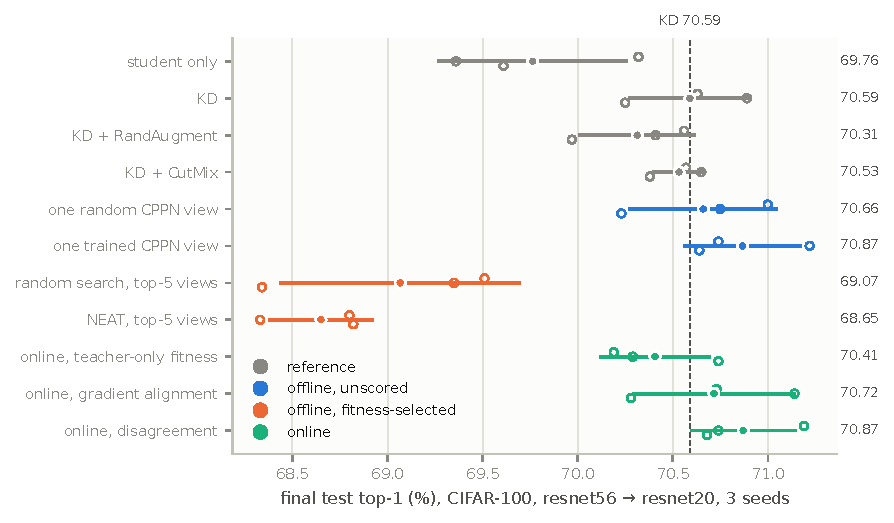
\includegraphics[width=\columnwidth]{figures/fig1_main_results.pdf}
\caption{Final test accuracy on resnet56 $\to$ resnet20 (hollow: seeds;
filled: mean $\pm$ std). Fitness-selected views (orange) fall well below KD
(dashed); unscored views (blue) and online variants (green) do not.}
\label{fig:main}
\end{figure}

The pattern holds on two further pairs (Figure~\ref{fig:generality}). On
wrn\_40\_2 $\to$ wrn\_16\_2, evolved views cost $1.57$ points ($p=0.049$)
while one random view is neutral ($+0.14$); on the cross-architecture pair
vgg13 $\to$ MobileNetV2 they cost $4.51$ points (seeds $-2.4$ to $-6.5$,
$p=0.06$) against $-0.66$ for one random view. Using the same fitness
online recovers most of the loss on every pair ($+1.35$, $p=0.047$ on WRN;
$+3.62$, $p=0.09$ on MobileNetV2).

\begin{figure}
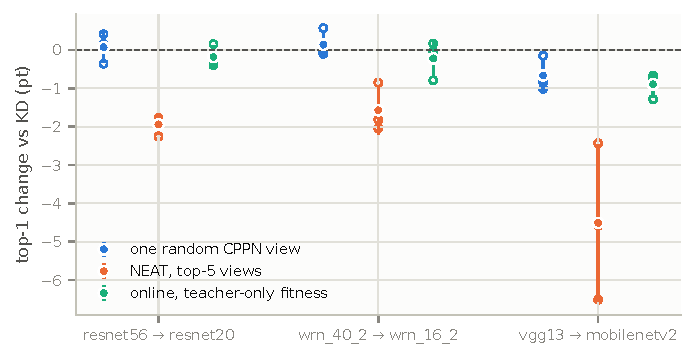
\includegraphics[width=\columnwidth]{figures/fig6_generality.pdf}
\caption{Change in final test accuracy relative to KD on three pairs.
Evolved views hurt on every pair, most on the weakest student.}
\label{fig:generality}
\end{figure}

% ---------------------------------------------------------------------------
\section{The fitness filters but does not rank}
\label{sec:fitness}

To see the fitness at the level of individual views, we built a bank of 40
genomes: 20 from a NEAT run and 20 from an equal-budget random search, at
evenly spaced fitness quantiles of each pool, all rescored on one shared
set of 1{,}024 probe images. Each view trained a resnet20 student for 60
epochs (the same schedule shape, two seeds), compared with KD on the same
schedule ($67.83\pm0.34$). Absolute effects on this short schedule are
larger than on the full one, so we interpret only rankings.

Two regimes appear (Figure~\ref{fig:fitness}a). Eleven views leave the
teacher with at most 39\% of its accuracy---the fitness's agreement gate is
closed for all of them---and are catastrophic, costing 5 to 19 points. The
other 29 lie within $-1.6$ to $+0.4$ points of KD. Over all 40 views the
fitness correlates positively with student benefit ($\rho=0.45$), but this
only reflects the gate separating the two regimes.

Inside the gate-open regime, among the 17 evolved views, a higher fitness
means a \emph{worse} student: $\rho=-0.61$ ($p=0.009$;
Figure~\ref{fig:fitness}b). The diversity term, which evolution maximizes,
is the driver: $\rho=-0.70$ ($p=0.002$; Figure~\ref{fig:fitness}c), and
$-0.52$ ($p=0.04$) after controlling for how much of the image the mask
keeps. The agreement term points the other way ($\rho=+0.65$). Once the
gate opens, the multiplicative fitness lets search trade agreement for
diversity, which is exactly the trade the student pays for. The diversity
result holds at every cutoff we tried; the fitness correlation depends on
one borderline view (with it included, $\rho=-0.36$, $p=0.15$). Comparing
each pool's five highest-fitness views reproduces the direction of the
full-length result: evolved $-0.55$ against random $-0.12$ ($p=0.055$).

\begin{figure*}
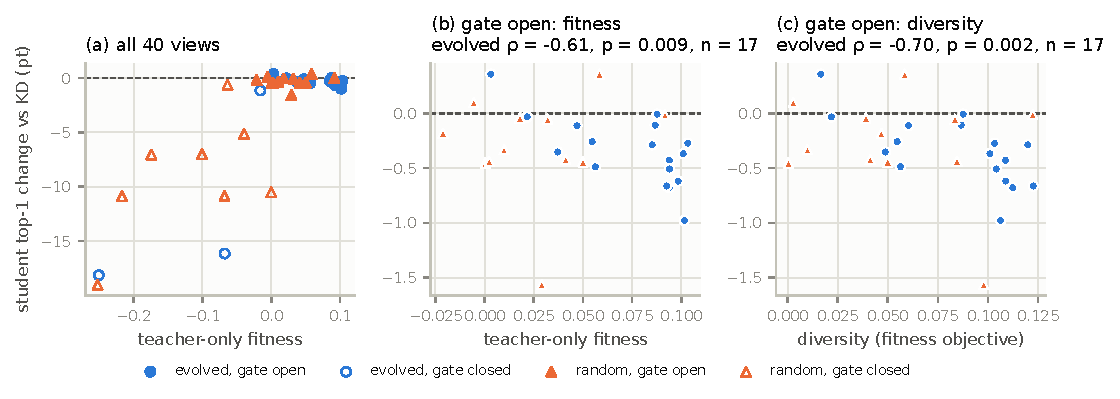
\includegraphics[width=\textwidth]{figures/fig3_fitness_study.pdf}
\caption{(a) Student accuracy change versus fitness for all 40 bank views;
hollow markers: the fitness's agreement gate is closed. (b, c) Gate-open
views only: among evolved views, fitness and its diversity term are
negatively correlated with student benefit.}
\label{fig:fitness}
\end{figure*}

The highest-fitness views are nearly identical: a mid-gray mask with one
thin bright stripe (Figure~\ref{fig:gallery}). Halving brightness and
adding a structured edge buys teacher-feature diversity cheaply. The most
harmful views are saturated color fields and high-frequency rings.

\begin{figure}
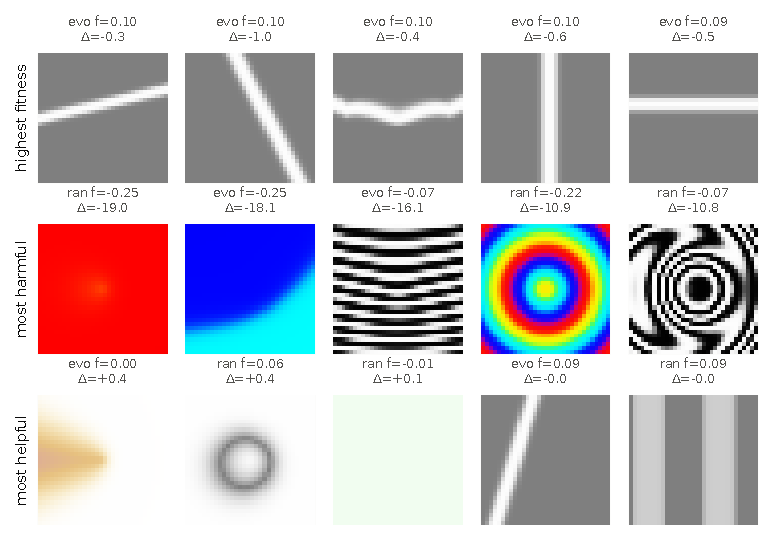
\includegraphics[width=\columnwidth]{figures/fig4_view_gallery.pdf}
\caption{Bank views: the five with the highest fitness, the five most
harmful and the five most helpful ($f$: fitness; $\Delta$: change versus
short-schedule KD).}
\label{fig:gallery}
\end{figure}

% ---------------------------------------------------------------------------
\section{What actually matters}
\label{sec:ablations}

We ablate the online method with a student-aware fitness---the KL
divergence between teacher and student on the view, counted only where the
teacher stays correct---on resnet56 $\to$ resnet20 (Figure~\ref{fig:ablations}).
This method itself reaches $70.87\pm0.28$, $+0.28$ over KD ($p=0.32$),
exactly matching one trained CPPN view; a second student-aware fitness
based on gradient alignment does no better ($70.72$). Selection, however
well informed, adds nothing measurable once views stop doing harm.

Re-evolution frequency (every 10 or 40 epochs), the random shift and flip,
and NEAT versus random search under the same fitness make no measurable
difference ($|\Delta|\le0.26$, $p\ge0.28$). Applying all five views to every
batch instead of sampling one costs $1.22$ points ($p=0.03$). This is the
configuration of the offline methods in Section~\ref{sec:harm}, so part of
their harm comes from how views are applied. Consistently, moving the
teacher-only fitness online with one view per batch recovers $1.76$ points
($p=0.002$).

\begin{figure}
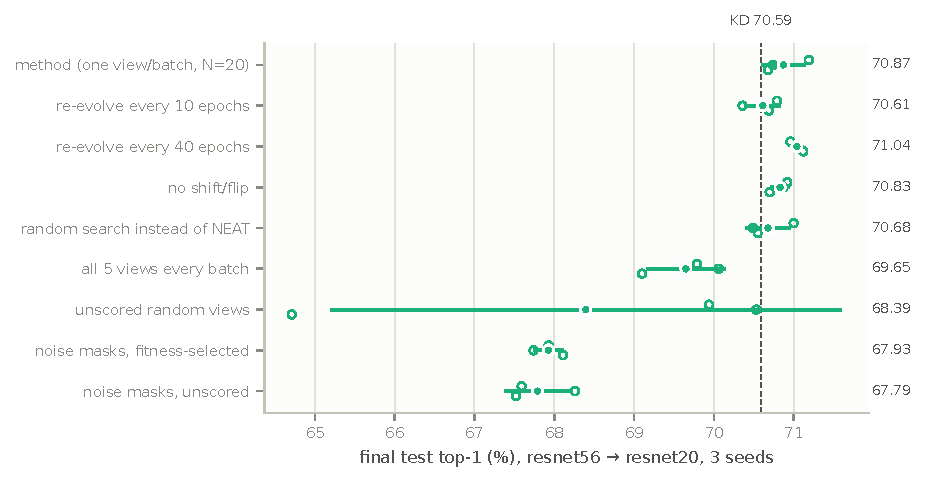
\includegraphics[width=\columnwidth]{figures/fig2_ablations.pdf}
\caption{Ablations of the online method on resnet56 $\to$ resnet20.}
\label{fig:ablations}
\end{figure}

Selection does matter as a safety filter. With unscored random views the
mean drops to $68.39\pm3.20$, and the training curves show why
(Figure~\ref{fig:refresh}): in all three seeds, test accuracy collapses
after late view refreshes---within ten epochs of the epoch-200 refresh it
falls from 70.7 to 59.6 and from 69.1 to 56.4 in two seeds, with single
epochs near 31\%---and recovers when the next refresh replaces the views. The final numbers
depend on which views happen to be active at the end. The filtered
method's curves stay flat.

\begin{figure}
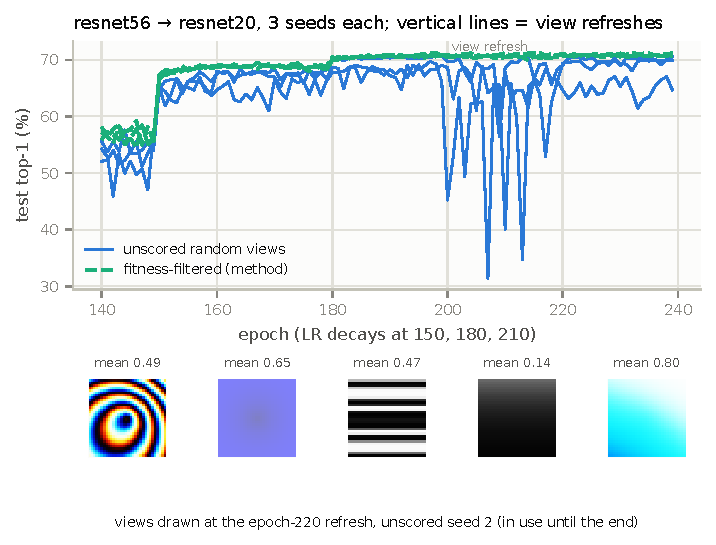
\includegraphics[width=\columnwidth]{figures/fig7_refresh_instability.pdf}
\caption{Test accuracy late in training with unscored random views (blue)
and the fitness-filtered method (green), three seeds each; bottom: the
views in use at the end of the seed with the lowest final accuracy.}
\label{fig:refresh}
\end{figure}

Finally, the CPPN family matters. Low-frequency noise masks cost $2.80$
points relative to KD ($p=0.001$), and selecting them with the same
student-aware fitness does not help ($67.93$ versus $67.79$, $p=0.63$),
while CPPN masks selected that way reach $70.87$ ($p<0.001$). Smooth CPPN
masks are benign where noise masks are not, and selection does not rescue
a bad family.

% ---------------------------------------------------------------------------
\section{Robustness and calibration}
\label{sec:robustness}

On CIFAR-100-C~\cite{hendrycks2019benchmarking} (mean over 15 corruptions
and five severities), robustness follows clean accuracy
(Figure~\ref{fig:robustness}): evolved views are the least robust on every
pair, by $2.49$, $0.89$ and $5.79$ points relative to KD on the three
pairs, so they do not trade clean accuracy for robustness. KD students are
markedly less calibrated than students trained alone (expected calibration
error~\cite{guo2017calibration} around 12\% versus 6.5\% on resnet20), and
any view lowers it---on MobileNetV2 from 18.3\% to about 10.4\% for both
harmful and benign views---so calibration does not distinguish good views
from bad ones.

\begin{figure*}
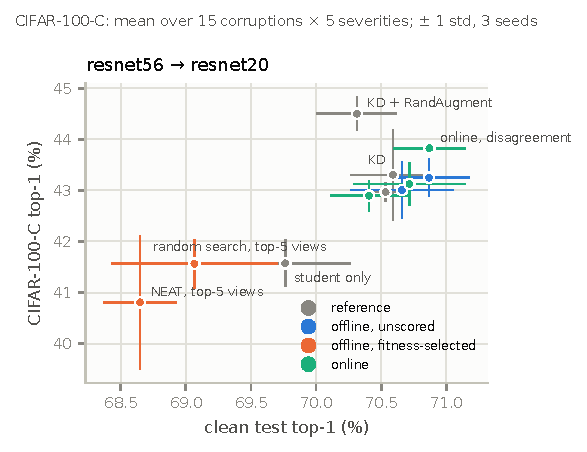
\includegraphics[width=\textwidth]{figures/fig5_robustness.pdf}
\caption{Clean versus corrupted (CIFAR-100-C) accuracy on three pairs.}
\label{fig:robustness}
\end{figure*}

% ---------------------------------------------------------------------------
\section{Discussion}
\label{sec:discussion}

\paragraph{Why the proxy fails.} The fitness rewards diversity subject to
agreement. The gate makes that constraint soft: once agreement clears
$\tau_{\mathrm{low}}$, a genome gains more by increasing diversity than it
loses by reducing agreement, and the views produced this way are the ones
that hurt the student. Diversity measured in a frozen teacher's feature
space is not the same thing as useful information for a student; the
cheapest ways to change those features (dimming, sharp edges, color
shifts) are not ways to teach.

\paragraph{Where to validate a proxy.} Over all views, the fitness looks
useful ($\rho=0.45$). Inside the region evolution occupies, it points the
wrong way. A sanity check on random samples would have passed this proxy;
only a check on the optimizer's own output exposes it.

\paragraph{Limitations.} One dataset (CIFAR-100), three seeds per
configuration, one mask operator (multiplicative), and a short-schedule
proxy for the view-level study. The negative fitness correlation depends
on one borderline view; the diversity correlation does not. The fourteen
revisions used an earlier, non-standard protocol.

% ---------------------------------------------------------------------------
\section{Conclusion}

A teacher-only fitness for evolved auxiliary views is a filter, not a
ranking: it rejects catastrophic views, but among the views evolution
produces, its objective term is anti-aligned with what the student needs.
Applying views one per batch matters more than selecting them, and student-
aware fitness functions did not change that. We expect the broader lesson
to transfer: validate a proxy fitness against the true objective in the
region the search actually reaches.

\begin{acks}
\todo{acknowledgments; compute: NJIT Wulver}
\end{acks}

\bibliographystyle{ACM-Reference-Format}
\bibliography{references}

\end{document}
